\title{The \textsc{ForSyDe-TikZ} library}
\author{
        George Ungureanu \\
                Department of Electronic Systems\\
        KTH---Royal Institute of Technology\\
        Stockholm, SWEDEN
}
\date{\today}

\documentclass[10pt]{article}
\usepackage[a4paper]{geometry}
\usepackage{forsyde-pc}
\usepackage[footnotesize]{caption}
\usepackage{hyperref}
\usepackage{enumitem}
\usepackage{marginnote}
\usepackage{listings}
\pgfplotsset{compat=1.9}


\newenvironment{optionslist}[0]{ 
\begin{list}{}{
	\setlength{\itemindent}{-10pt}
%	\setlength{\topsep}{0pt}
	\setlength{\itemsep}{0pt}
	\setlength{\parsep}{0pt}
}}{\end{list}}
\newcommand\bookmark[1]{\marginpar{\ttfamily #1}}
\tikzset{% 
    anch/.style={circle, draw=none, fill=red, inner sep=0pt, minimum size=3pt},
    label/.style={font=\ttfamily\scriptsize}
}
\lstset{
  basicstyle=\footnotesize\ttfamily,
  numbers=left,
  frame=single,
  numberstyle=\tiny\color{black!30},
  commentstyle=\color{blue}\textit,
  stringstyle=\color{magenta}\textit,
  flexiblecolumns=false,
  basewidth={0.5em,0.45em},
  breaklines=true,
  language={[LaTeX]TeX},
  texcsstyle=*\color{red}\bfseries,
  keywordstyle=\color{blue}\bfseries,
  morekeywords={tikzpicture,document},
  moretexcs={crossed,standard,interface,basic,cluster,node,path},
}




\begin{document}
\maketitle
\reversemarginpar

\begin{abstract}
This document is the reference manual for using the \texttt{forsyde-tikz} and \texttt{forsyde-pc} packages.  All API features are documented here.
\end{abstract}

\section{Introduction}

\textsc{ForSyDe-TikZ} is a collection \textsc{TikZ} \& \textsc{PGF} graphical basics and environment macros for plotting process networks in \textsc{ForSyDe}. \textsc{ForSyDe} is a high-level design methodology aiming at synthesizing correct-by-construction systems using formal means. For more information check  \url{https://forsyde.ict.kth.se/trac}.

This library provides two main packages. \texttt{forsyde-tikz} provides graphical basics and macros for creating custom process constructors whereas \texttt{forsyde-pc} contains helper macros for drawing the process constructors defined in \textsc{ForSyDe} at the time of writing this document.

\section{Installation}

The contents of \texttt{src} are to be copied on your local machine, ideally in your LaTeX  project folder. The package is loaded by compiling your document with the \texttt{TEXINPUTS} variable set to your installation path, or by copying all of the package files in your document's root folder or any LaTeX  standard loading paths. 

\section{Getting started}

A \textsc{ForSyDe} process network is drawn like any other \textsc{TikZ} figure, inside a \texttt{tikzpicture} environment. The \texttt{options} provided are key variables defined by the \texttt{tikz} package. \bookmark{environment}

\begin{verbatim}
	\begin{tikzpicture}[options]
		content...
	\end{tikzpicture}
\end{verbatim}

The following figure can be produced by either customizing every element with the basics provided in \texttt{forsyde-tiks}:

\begin{figure}[htb]\centering
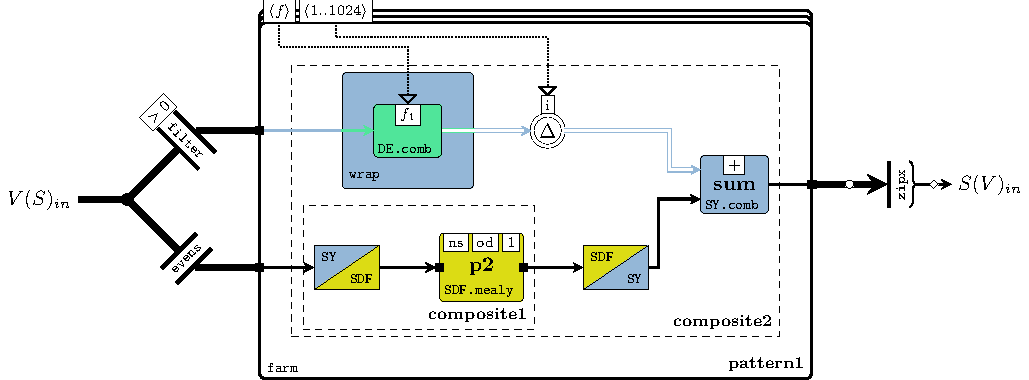
\includegraphics[width=\textwidth]{figs/example-forsyde-tikz}
\end{figure}

\lstinputlisting{figs/example-forsyde-tikz.tex}

\section{The \texttt{forsyde-tikz} package}

The \texttt{forsyde-tikz} package is included with

\begin{verbatim}
	\usepackage{forsyde-tikz}
\end{verbatim}

Apart from the standard keys, \texttt{forsyde-tikz} provides the following variables:\bookmark{environment variables}
 \begin{optionslist}
\item \texttt{nomoccolor} : disables process coloring according to their MoC.
\item \texttt{nomoclabel} : disables process labeling according to their MoC.
\item \texttt{label style=} : font style for the process type labels. Default is \texttt{\char`\\ textbf}.
\item \texttt{type style=} : font style for the process name labels. Default is \texttt{\char`\\ scriptsize\char`\\textit}.
\item \texttt{function style=} : font style for the functions. Default is \texttt{\char`\\ scriptsize}.
\item \texttt{global scale=} : scale of the picture. Should be used instead of the \textsc{TikZ} \texttt{scale}.
\end{optionslist}

\subsection{Main nodes}

Leaf processes are basic nodes in a process network. They can be drawn either using a standad symbol or using a custom shape. One special case of leaf process is the interface. \texttt{forsyde-tikz} provides a command for creating each of these nodes: \texttt{\char`\\leafstd} for standard symbol, \texttt{\char`\\standard} for custom shape or \texttt{\char`\\interface} for interface.\\

\hspace{1pt}\bookmark{\char`\\standard[shape=leaf,options]\{id\}\{position\}\{label\}}

\begin{optionslist}
\item \texttt{moc=[none,ct,de,sy,sdf]} the model of computation. Defaut is \texttt{none}.
\item \texttt{type=} the process type. It will be shown below the label.
\item \texttt{ni=[0..10]} the number of input ports. Default is 1.
\item \texttt{no=[0..10]} the number of output ports. Default is 1.
\item \texttt{nf=[0..4]} the number of passed functions. Default is 1.
\item \texttt{f1=} the first function label. It will be shown in the appropriate place in case \texttt{nf > 0}. Default is $f_1$.
\item \texttt{f2=} the second function label. It will be shown in the appropriate place in case \texttt{nf > 1}. Default is $f_2$.
\item \texttt{f3=} the third function label. It will be shown in the appropriate place in case \texttt{nf > 2}. Default is $f_3$.
\item \texttt{f4=} the fourth function label. It will be shown in the appropriate place in case \texttt{nf > 3}. Default is $f_4$.
\item\texttt{inner sep=} vertical distance between the function labels, process label and process type. Default is \texttt{10pt}.
\item\texttt{reverse} toggle switch which determines the orientation of the input/output ports. Default is off (inputs to the left and outputs to the right).
\end{optionslist}

% \begin{lstlisting}
% \standard[shape=leaf,moc=ct, type=comb, nf=4, ni=2, no=3, f1=$x/y$, f2=$a+b$] {p1}{0,0}{P1};
% \standard[shape=leaf,moc=sy, reverse, type=comb, nf=4, ni=2, no=5, f2=$a+b$,inner sep=15pt] {p2}{6,0}{P2};
% \end{lstlisting}
% \begin{figure}[htb!]\centering
% \begin{tikzpicture}[]
% \standard[shape=leaf,moc=ct, type=comb, nf=4, ni=2, no=3, f1=$x/y$, f2=$a+b$] {p1}{0,0}{P1};
% \standard[shape=leaf,moc=sy, reverse, type=comb, nf=4, ni=2, no=5, f2=$a+b$,inner sep=15pt] {p2}{6,0}{P2};

% \node[anch] (a) at (p1.i1) {}; \node[label, anchor=east] (l) at (a.west) {\texttt{p1.i1}};
% \node[anch] (a) at (p1.i2) {}; \node[label, anchor=east] (l) at (a.west) {\texttt{p1.i2}};
% \node[anch] (a) at (p1.o1) {}; \node[label, anchor=west] (l) at (a.east) {\texttt{p1.o1}};
% \node[anch] (a) at (p1.o2) {}; \node[label, anchor=west] (l) at (a.east) {\texttt{p1.o2}};
% \node[anch] (a) at (p1.o3) {}; \node[label, anchor=west] (l) at (a.east) {\texttt{p1.o3}};
% \node[anch] (a) at (p1-f.i1) {}; \node[label, anchor=west, rotate=90] (l) at (a.north) {\texttt{p1-f.i1}};
% \node[anch] (a) at (p1-f.i2) {}; \node[label, anchor=west, rotate=90] (l) at (a.north) {\texttt{p1-f.i2}};
% \node[anch] (a) at (p1-f.i3) {}; \node[label, anchor=west, rotate=90] (l) at (a.north) {\texttt{p1-f.i3}};
% \node[anch] (a) at (p1-f.i4) {}; \node[label, anchor=west, rotate=90] (l) at (a.north) {\texttt{p1-f.i4}};

% \node[anch] (a) at (p2.i1) {}; \node[label, anchor=west] (l) at (a.east) {\texttt{p2.i1}};
% \node[anch] (a) at (p2.i2) {}; \node[label, anchor=west] (l) at (a.east) {\texttt{p2.i2}};
% \node[anch] (a) at (p2.o1) {}; \node[label, anchor=east] (l) at (a.west) {\texttt{p2.o1}};
% \node[anch] (a) at (p2.o2) {}; \node[label, anchor=east] (l) at (a.west) {\texttt{p2.o2}};
% \node[anch] (a) at (p2.o3) {}; \node[label, anchor=east] (l) at (a.west) {\texttt{p2.o3}};
% \node[anch] (a) at (p2.o4) {}; \node[label, anchor=east] (l) at (a.west) {\texttt{p2.o4}};
% \node[anch] (a) at (p2.o5) {}; \node[label, anchor=east] (l) at (a.west) {\texttt{p2.o5}};
% \node[anch] (a) at (p2-f.i1) {}; \node[label, anchor=west, rotate=90] (l) at (a.north) {\texttt{p2-f.i1}};
% \node[anch] (a) at (p2-f.i2) {}; \node[label, anchor=west, rotate=90] (l) at (a.north) {\texttt{p2-f.i2}};
% \node[anch] (a) at (p2-f.i3) {}; \node[label, anchor=west, rotate=90] (l) at (a.north) {\texttt{p2-f.i3}};
% \node[anch] (a) at (p2-f.i4) {}; \node[label, anchor=west, rotate=90] (l) at (a.north) {\texttt{p2-f.i4}};
% \end{tikzpicture}
% \end{figure}

% \hspace{1pt}\bookmark{\char`\\standard[options]\{id\}\{position\}}

% \begin{optionslist}
% \item \texttt{moc=[none,ct,de,sy,sdf]} the model of computation. Defaut is \texttt{none}.
% \item \texttt{shape=} the node shape. For a list of available shapes check \autoref{appendix_shapes}.
% \item \texttt{ni=[0..10]} the number of input ports. Default is 1.
% \item \texttt{no=[0..10]} the number of output ports. Default is 1.
% \item \texttt{minimum height=} the minimum height of a node. Default is \texttt{15pt}.
% \item\texttt{reverse} toggle switch which determines the orientation of the input/output ports. Default is off (inputs to the left and outputs to the right).
% \item\texttt{reverse shape} toggle switch which determines the orientation of the chosen shape. Default is off.
% \end{optionslist}

% \begin{lstlisting}
% \standard[moc=de, shape=zip shape, reverse, reverse shape, ni=2, no=1] {lc}{5,0};
% \end{lstlisting}
% \begin{figure}[htb!]\centering
% \begin{tikzpicture}[]
% \standard[moc=de, shape=zip shape, reverse, reverse shape, ni=2, no=1] {lc}{5,0};

% \node[anch] (a) at (lc.i1) {}; \node[label, anchor=west] (l) at (a.east) {\texttt{lc.i1}};
% \node[anch] (a) at (lc.i2) {}; \node[label, anchor=west] (l) at (a.east) {\texttt{lc.i2}};
% \node[anch] (a) at (lc.o1) {}; \node[label, anchor=east] (l) at (a.west) {\texttt{lc.o1}};
% \end{tikzpicture}
% \end{figure}

% \hspace{1pt}\bookmark{\char`\\interface[options]\{id\}\{position\}}
% \begin{optionslist}
% \item \texttt{mocin=[none,ct,de,sy,sdf]} the input MoC. Defaut is \texttt{none}.
% \item \texttt{mocin=[none,ct,de,sy,sdf]} the output MoC. Defaut is \texttt{none}.
% \item\texttt{reverse} toggle switch which determines the orientation of the input/output ports. Default is off (inputs to the left and outputs to the right).
% \end{optionslist}

% \begin{lstlisting}
% \interface[mocin=ct, mocout=de] {di}{0,0};
% \interface[mocin=ct, mocout=de, reverse] {direv}{5,0};
% \end{lstlisting}

% \begin{figure}[htb!]\centering
% \begin{tikzpicture}[]
% \interface[mocin=ct, mocout=de] {di}{0,0};
% \interface[mocin=ct, mocout=de, reverse] {direv}{5,0};

% \node[anch] (a) at (di.i1) {}; \node[label, anchor=east] (l) at (a.west) {\texttt{di.i1}};
% \node[anch] (a) at (di.o1) {}; \node[label, anchor=west] (l) at (a.east) {\texttt{di.o1}};

% \node[anch] (a) at (direv.i1) {}; \node[label, anchor=west] (l) at (a.east) {\texttt{direv.i1}};
% \node[anch] (a) at (direv.o1) {}; \node[label, anchor=east] (l) at (a.west) {\texttt{direv.o1}};
% \end{tikzpicture}
% \end{figure}

% \hspace{1pt}\bookmark{\char`\\compositestd[options]\{id\}\{list~of~clustered~nodes\}\{label\}}

% \hspace{1pt}\bookmark{\char`\\compositebbox[options]\{id\}\{position\}\{label\}}


% \begin{optionslist}
% \item \texttt{ni=[0..10]} the number of input ports. Default is 1.
% \item \texttt{no=[0..10]} the number of output ports. Default is 1.
% \item\texttt{inner xsep=} the distance between the outermost clustered nodes and the composite box edge. Default is 15pt.
% \item\texttt{inner ysep=} the distance between the outermost clustered nodes and the composite box edge. Default is 15pt.
% \item\texttt{reverse} toggle switch which determines the orientation of the input/output ports. Default is off (inputs to the left and outputs to the right).
% \end{optionslist}

% \begin{lstlisting}
% \compositebbox[ni=1, no=1]                 {bb}  {0,0} {BlackBox};
% \leafstd      [nf=0, inner sep=3pt]        {dm1} {8,-0.5} {Dummy1};
% \leafstd      [nf=0, inner sep=3pt]        {dm2} {8,0.5} {Dummy2};
% \compositestd [ni=2, no=3, inner xsep=35pt]{cp1} {(bb)} {CP1};
% \compositestd [ni=2, no=3, reverse]        {cp2} {(dm1)(dm2)} {CP2};
% \end{lstlisting}

% \begin{figure}[htb!]\centering
% \begin{tikzpicture}[global scale=.93]
% \compositebbox[ni=1, no=1] {bb} {0,0} {BlackBox};
% \standard[shape=leaf,nf=0, inner sep=3pt] {dm1} {8,-0.5} {Dummy1};
% \standard[shape=leaf,nf=0, inner sep=3pt] {dm2} {8,0.5} {Dummy2};
% \compositestd[ni=2, no=3, inner xsep=35pt] {cp1} {(bb)} {CP1};
% \compositestd[ni=2, no=3, reverse] {cp2} {(dm1)(dm2)} {CP2};

% \node[anch] (a) at (bb.i1) {}; \node[label, anchor=east] (l) at (a.west) {\texttt{bb.i1}};
% \node[anch] (a) at (bb.o1) {}; \node[label, anchor=west] (l) at (a.east) {\texttt{bb.o1}};

% \node[anch] (a) at (cp1.i1) {}; \node[label, anchor=east] (l) at (a.west) {\texttt{cp1.i1}};
% \node[anch] (a) at (cp1.i2) {}; \node[label, anchor=east] (l) at (a.west) {\texttt{cp1.i2}};
% \node[anch] (a) at (cp1.o1) {}; \node[label, anchor=west] (l) at (a.east) {\texttt{cp1.o1}};
% \node[anch] (a) at (cp1.o2) {}; \node[label, anchor=west] (l) at (a.east) {\texttt{cp1.o2}};
% \node[anch] (a) at (cp1.o3) {}; \node[label, anchor=west] (l) at (a.east) {\texttt{cp1.o3}};

% \node[anch] (a) at (cp2.i1) {}; \node[label, anchor=west] (l) at (a.east) {\texttt{cp2.i1}};
% \node[anch] (a) at (cp2.i2) {}; \node[label, anchor=west] (l) at (a.east) {\texttt{cp2.i2}};
% \node[anch] (a) at (cp2.o1) {}; \node[label, anchor=east] (l) at (a.west) {\texttt{cp2.o1}};
% \node[anch] (a) at (cp2.o2) {}; \node[label, anchor=east] (l) at (a.west) {\texttt{cp2.o2}};
% \node[anch] (a) at (cp2.o3) {}; \node[label, anchor=east] (l) at (a.west) {\texttt{cp2.o3}};
% \end{tikzpicture}
% \end{figure}

% \vspace{20pt}
% \hspace{1pt}\bookmark{\char`\\patterncluster[options]\{id\}\{list~of~clustered~nodes\}\{label\}}

% \begin{optionslist}
% \item \texttt{type=} the process type label.
% \item \texttt{shape=} the cluster node shape. Default is \texttt{dp shape}. For a list of shapes check \autoref{appendix_shapes}
% \item \texttt{ni=[0..10]} the number of input ports. Default is 1.
% \item \texttt{no=[0..10]} the number of output ports. Default is 1.
% \item \texttt{nf=[0..4]} the number of passed functions. Default is 1.
% \item \texttt{f1=} the first function label. It will be shown in the appropriate place in case \texttt{nf > 0}. Default is $\langle f_1 \rangle$.
% \item \texttt{f2=} the second function label. It will be shown in the appropriate place in case \texttt{nf > 1}. Default is $\langle f_2 \rangle$.
% \item \texttt{f3=} the third function label. It will be shown in the appropriate place in case \texttt{nf > 2}. Default is $\langle f_3 \rangle$.
% \item \texttt{f4=} the fourth function label. It will be shown in the appropriate place in case \texttt{nf > 3}. Default is $\langle f_4 \rangle$.
% \item\texttt{inner xsep=} the distance between the outermost clustered nodes and the composite box X edge. Default is 15pt.
% \item\texttt{inner ysep=} the distance between the outermost clustered nodes and the composite box Y edge. Default is 18pt.
% \item\texttt{reverse} toggle switch which determines the orientation of the input/output ports. Default is off (inputs to the left and outputs to the right).
% \item\texttt{reverse shape} toggle switch which determines the orientation of the chosen shape. Default is off.
% \end{optionslist}

% \begin{lstlisting}
% \standard[shape=leaf,nf=0, inner sep=3pt] {dm1} {0,-0.5} {Dummy 1};
% \standard[shape=leaf,nf=0, inner sep=3pt] {dm2} {0,0.5} {Dummy 2};
% \standard[shape=leaf,nf=0, inner sep=3pt] {dm3} {6,0} {Dummy 3};
% \patterncluster[ni=2, no=2, nf=2, shape=dp shape, type=farm2, inner ysep=25pt] 
% 	{dp} {(dm1)(dm2)} {Farm1};
% \patterncluster[ni=1, no=2, nf=3, f3=scanld (+), shape=pipe shape, type=pipe3, reverse, inner ysep=25pt] 
% 	{pr} {(dm3)} {PipeRev1};
% \end{lstlisting}

% \begin{figure}[htb!]\centering
% \begin{tikzpicture}
% \standard[shape=leaf,nf=0, inner sep=3pt] {dm1} {0,-0.5} {Dummy 1};
% \standard[shape=leaf,nf=0, inner sep=3pt] {dm2} {0,0.5} {Dummy 2};
% \standard[shape=leaf,nf=0, inner sep=3pt] {dm3} {6,0} {Dummy 3};
% \patterncluster[ni=2, no=2, nf=2, shape=dp shape, type=farm2, inner ysep=25pt] 
% 	{dp} {(dm1)(dm2)} {Farm1};
% \patterncluster[ni=1, no=2, nf=3, f3=scanld (+), shape=pipe shape, type=pipe3, reverse, inner ysep=25pt] 
% 	{pr} {(dm3)} {PipeRev1};

% \node[anch] (a) at (dp.i1) {}; \node[label, anchor=east] (l) at (a.west) {\texttt{dp.i1}};
% \node[anch] (a) at (dp.i2) {}; \node[label, anchor=east] (l) at (a.west) {\texttt{dp.i2}};
% \node[anch] (a) at (dp.o1) {}; \node[label, anchor=west] (l) at (a.east) {\texttt{dp.o1}};
% \node[anch] (a) at (dp.o2) {}; \node[label, anchor=west] (l) at (a.east) {\texttt{dp.o2}};
% \node[anch] (a) at (dp-f.i1) {}; \node[label, anchor=west, rotate=90] (l) at (a.north) {\texttt{dp-f.i1}};
% \node[anch] (a) at (dp-f.i2) {}; \node[label, anchor=west, rotate=90] (l) at (a.north) {\texttt{dp-f.i2}};
% \node[anch] (a) at (dp-f.o1) {}; \node[label, anchor=west, rotate=-45] (l) at (a.north) {\texttt{dp-f.o1}};
% \node[anch] (a) at (dp-f.o2) {}; \node[label, anchor=west, rotate=-45] (l) at (a.north) {\texttt{dp-f.o2}};

% \node[anch] (a) at (pr.i1) {}; \node[label, anchor=west] (l) at (a.east) {\texttt{pr.i1}};
% \node[anch] (a) at (pr.o1) {}; \node[label, anchor=east] (l) at (a.west) {\texttt{pr.o1}};
% \node[anch] (a) at (pr.o2) {}; \node[label, anchor=east] (l) at (a.west) {\texttt{pr.o2}};
% \node[anch] (a) at (pr-f.i1) {}; \node[label, anchor=west, rotate=90] (l) at (a.north) {\texttt{pr-f.i1}};
% \node[anch] (a) at (pr-f.i2) {}; \node[label, anchor=west, rotate=90] (l) at (a.north) {\texttt{pr-f.i2}};
% \node[anch] (a) at (pr-f.i3) {}; \node[label, anchor=west, rotate=90] (l) at (a.north) {\texttt{pr-f.i3}};
% \node[anch] (a) at (pr-f.o1) {}; \node[label, anchor=west, rotate=-45] (l) at (a.north) {\texttt{pr-f.o1}};
% \node[anch] (a) at (pr-f.o2) {}; \node[label, anchor=west, rotate=-45] (l) at (a.north) {\texttt{pr-f.o2}};
% \node[anch] (a) at (pr-f.o3) {}; \node[label, anchor=west, rotate=-45] (l) at (a.north) {\texttt{pr-f.o3}};
% \end{tikzpicture}
% \end{figure}

% \hspace{1pt}\bookmark{\char`\\patternnodestd[options]\{id\}\{position\}}

% \hspace{1pt}\bookmark{\char`\\patternnodecustom[options]\{id\}\{position\}}

% \begin{optionslist}
% \item \texttt{type=} type label.
% \item \texttt{inner shape=} the inner shape. Default is \texttt{noinner}. For a list of available shapes check \autoref{appendix_shapes}.
% \item \texttt{outer shape=} the outer shape. Default is \texttt{transition shape v1gv1}. For a list of available shapes check \autoref{appendix_shapes}.
% \item \texttt{ni=[0..10]} the number of input ports. Default is 1.
% \item \texttt{no=[0..10]} the number of output ports. Default is 1.
% \item \texttt{nf=[0..4]} the number of passed functions. Default is 1.
% \item \texttt{f1=} the first function label. It will be shown in the appropriate place in case \texttt{nf > 0}. Default is $f_1$.
% \item \texttt{f2=} the second function label. It will be shown in the appropriate place in case \texttt{nf > 1}. Default is $f_2$.
% \item \texttt{f3=} the third function label. It will be shown in the appropriate place in case \texttt{nf > 2}. Default is $f_3$.
% \item \texttt{f4=} the fourth function label. It will be shown in the appropriate place in case \texttt{nf > 3}. Default is $f_4$.
% \item\texttt{reverse} toggle switch which determines the orientation of the input/output ports. Default is off (inputs to the left and outputs to the right).
% \item\texttt{reverse shape} toggle switch which determines the orientation of the chosen shape. Default is off.
% \end{optionslist}

% \begin{lstlisting}
% \patternnodecustom[outer shape=transition shape s1v1] {a}{0,0};
% \patternnodestd   [ni=2, nf=1, f1=$f(i)$, type=distribute, outer shape=transition shape v2v1] {b}{3,0};
% \patternnodecustom[inner shape=custom conduit i8o3] {c}{6,0};
% \patternnodecustom[inner shape=custom conduit i8o8, outer shape=transition shape v1gv1, reverse] {d}{9,0};
% \end{lstlisting}

% \begin{figure}[htb!]\centering
% \begin{tikzpicture}
% \patternnodecustom[outer shape=transition shape s1v1] {a}{0,0};
% \patternnodestd   [ni=2, nf=1, f1=$f(i)$, type=distribute, outer shape=transition shape v2v1] {b}{3,0};
% \patternnodecustom[inner shape=custom conduit i8o3] {c}{6,0};
% \patternnodecustom[inner shape=custom conduit i8o8, outer shape=transition shape v1gv1, reverse] {d}{9,0};

% \node[anch] (x) at (a.i1) {}; \node[label, anchor=east] (l) at (x.west) {\texttt{a.i1}};
% \node[anch] (x) at (a.o1) {}; \node[label, anchor=west] (l) at (x.east) {\texttt{a.o1}};
% \node[anch] (x) at (b.i1) {}; \node[label, anchor=east] (l) at (x.west) {\texttt{b.i1}};
% \node[anch] (x) at (b.i2) {}; \node[label, anchor=east] (l) at (x.west) {\texttt{b.i2}};
% \node[anch] (x) at (b.o1) {}; \node[label, anchor=west] (l) at (x.east) {\texttt{b.o1}};
% \foreach \i in {0,1,...,2} {	\node[anch] (x) at (c-c.vo\i) {}; \node[label, anchor=west] (l) at (x.east) {\texttt{c-c.vo\i}};}
% \foreach \i in {0,1,...,7} {
% 	\node[anch] (x) at (c-c.vi\i) {}; \node[label, anchor=east] (l) at (x.west) {\texttt{c-c.vi\i}};
% 	\node[anch] (x) at (d-c.vo\i) {}; \node[label, anchor=east] (l) at (x.west) {\texttt{d-c.vo\i}};

% 	\node[anch] (x) at (d-c.vi\i) {}; \node[label, anchor=west] (l) at (x.east) {\texttt{d-c.vi\i}};
% }
% \end{tikzpicture}
% \end{figure}

% \subsection{Paths}

% Data flow in ForSyDe is represented with paths. \textsc{ForSyDe-TikZ} provides three macros for drawing signals (\texttt{\string\signal}), vectors (\texttt{\string\vector}) or function interfaces (\texttt{\string\function}) between process anchors. \\


% \hspace{1pt}\bookmark{\char`\\signal[options]~(from)~shape~(to);}

% \hspace{1pt}\bookmark{\char`\\vector[options]~(from)~shape~(to);}

% \begin{optionslist}
% \item \texttt{moc=[none,ct,de,sy,sdf]} the model of computation. Defaut is \texttt{none}.
% \item \texttt{token=[scalar,vector,function,scalarAE,vectorAE,functionAE]} draws symbols for depicting the token structure of ForSyDe signals or vectors. Function paths will ignore this key. To draw tuple structures you have to separate token keywords by \texttt{-} (dash). E.g.: 3-tuple of scalar, absent extended vector and function can be drawn with \texttt{token=scalar-vectorAE-function}.
% \item \texttt{token pos=[0.0 .. 1.0]} the position between the start node/anchor and the end node/anchor where the token begins to be drawn.
% \item \texttt{-|-=[0.0 .. 1.0]} will create a horizontal-vertical-horizontal spline in the path. It may be accompanied by a number which determines the position of the 90 degree angle.
% \item \texttt{|-|=[0.0 .. 1.0]} will create a vertical-horizontal-vertical spline in the path. It may be accompanied by a number which determines the position of the 90 degree angle.
% \item \texttt{-|-=[0.0 .. 1.0]} will create a horizontal-vertical-horizontal spline in the path. It may be accompanied by a number which determines the position of the 90 degree angle.
% \item \texttt{-|-|=[0.0 .. 1.0]} will create a horizontal-vertical-horizontal-vertical spline in the path. It may be accompanied by a number which determines the position of the 90 degree angle.
% \item \texttt{-|-|-=[0.0 .. 1.0]:[0.0 .. 1.0]} will create a horizontal-vertical-horizontal-vertical-horizontal spline in the path. It may be accompanied by two numbers  separated by \texttt{:} which determine the position of the 90 degree angles.
% \item \texttt{|-|-|=[0.0 .. 1.0]:[0.0 .. 1.0]} will create a vertical-horizontal-vertical-horizontal-vertical spline in the path. It may be accompanied by two numbers  separated by \texttt{:} which determine the position of the 90 degree angles.
% \item \texttt{deviation=} is a length representing the deviation from the straight path in case of complex splines (\texttt{-|-|},\texttt{-|-|-} and \texttt{|-|-|}).
% \end{optionslist}

% \begin{lstlisting}
% \signal[]                                     (0,2)  ->  (1.5,2); 
% \signal[moc=ct, token=vectorAE-functionAE]    (2,2)  <-  (3.5,2);
% \signal[moc=sy, -|-|-=0.2:0.6, deviate=-10pt] (4,2)  p->p (5.5,2);
% \signal[token=scalarAE, -|-]                  (6,1.7) ->p (7.5,2.3);
% \signal[token pos=0.2, token=scalar-vector]   (8,2)  ->  (9.5,2);
% \end{lstlisting}

% \begin{figure}[htb!]\centering
% \begin{tikzpicture}[]
% 	\signal[]                                     (0,2)  ->  (1.5,2); 
% 	\signal[moc=ct, token=vectorAE-functionAE]    (2,2)  <-  (3.5,2);
% 	\signal[moc=sy, -|-|-=0.2:0.6, deviate=-10pt] (4,2)  p->p (5.5,2);
% 	\signal[token=scalarAE, -|-]                  (6,1.7) ->p (7.5,2.3);
% 	\signal[token pos=0.2, token=scalar-vector]   (8,2)  ->  (9.5,2);
% \end{tikzpicture}
% \end{figure}

% \begin{lstlisting}
% \vector[token=scalar-scalar-scalar-scalar] (0,1) p->p (2,1);	
% \vector[moc=sdf]                           (3,1) p->p (5,1);
% \vector[token=vectorAE, token pos=0.35]    (6,1) p->p (8,1);
% \end{lstlisting}

% \begin{figure}[htb!]\centering
% \begin{tikzpicture}[]
% 	\vector[token=scalar-scalar-scalar-scalar] (0,1) p->p (2,1);	
% 	\vector[moc=sdf]                           (3,1) p->p (5,1);
% 	\vector[token=vectorAE, token pos=0.35]    (6,1) p->p (8,1);
% \end{tikzpicture}
% \end{figure}


% \hspace{1pt}\bookmark{\char`\\function[options]~(from)~shape~(to);}
% \begin{optionslist}
% \item \texttt{-|-=[0.0 .. 1.0]} will create a horizontal-vertical-horizontal spline in the path. It may be accompanied by a number which determines the position of the 90 degree angle.
% \item \texttt{|-|=[0.0 .. 1.0]} will create a vertical-horizontal-vertical spline in the path. It may be accompanied by a number which determines the position of the 90 degree angle.
% \item \texttt{-|-=[0.0 .. 1.0]} will create a horizontal-vertical-horizontal spline in the path. It may be accompanied by a number which determines the position of the 90 degree angle.
% \item \texttt{-|-|=[0.0 .. 1.0]} will create a horizontal-vertical-horizontal-vertical spline in the path. It may be accompanied by a number which determines the position of the 90 degree angle.
% \item \texttt{-|-|-=[0.0 .. 1.0]:[0.0 .. 1.0]} will create a horizontal-vertical-horizontal-vertical-horizontal spline in the path. It may be accompanied by two numbers  separated by \texttt{:} which determine the position of the 90 degree angles.
% \item \texttt{|-|-|=[0.0 .. 1.0]:[0.0 .. 1.0]} will create a vertical-horizontal-vertical-horizontal-vertical spline in the path. It may be accompanied by two numbers  separated by \texttt{:} which determine the position of the 90 degree angles.
% \item \texttt{deviation=} is a length representing the deviation from the straight path in case of complex splines (\texttt{-|-|},\texttt{-|-|-} and \texttt{|-|-|}).
% \end{optionslist}

% \begin{lstlisting}
% \function[] (0,0) -> (2,0);
% \function[|-|=.6] (3,.5) fi-> (4,-.5);
% \function[|-|-|] (5,.5) <- (5,-.5);
% \end{lstlisting}

% \begin{figure}[htb!]\centering
% \begin{tikzpicture}[]
% 	\function[] (0,0) -> (2,0);
% 	\function[|-|=.6] (3,.5) fi-> (4,-.5);
% 	\function[|-|-|] (5,.5) <- (5,-.5);
% \end{tikzpicture}
% \end{figure}

% \subsection{Miscellaneous functions}

% Following is a list of miscellaneous functions and environments provided for user convenience:\\

% \hspace{1pt}\bookmark{\texttt{\string\textleftof\{node\}\{text\}}}

% \hspace{1pt}\bookmark{\texttt{\string\textrightof\{node\}\{text\}}}

% \hspace{1pt}\bookmark{\texttt{\string\textaboveof\{node\}\{text\}}}

% \hspace{1pt}\bookmark{\texttt{\string\textbelowof\{node\}\{text\}}}


% \subsection{Further customizing the environment}

% The following commands can be used in the document preamble for changing environment variables.
% \begin{lstlisting}
% % Colors
% \renewcommand{\defaultdrawcolor}{[color]}
% \renewcommand{\defaultfillcolor}{[color]}
% \definecolor{sycolor}{[coord sys]}{[color coord]}
% \definecolor{ctcolor}{[coord sys]}{[color coord]}
% \definecolor{decolor}{[coord sys]}{[color coord]}
% \definecolor{sdfcolor}{[coord sys]}{[color coord]}
% \definecolor{blackboxcolor}{[coord sys]}{[color coord]}}
% % line widths
% \pgfmathsetlength{\sepq}{[size]}           % small inter-node separation 
% \renewcommand{\compositelinewidth}{[size]}
% \renewcommand{\skeletonlinewidth}{[size]}  % parallel processes line width
% \renewcommand{\signalpathlinewidth}{[size]}
% \renewcommand{\functionpathlinewidth}{[size]}
% \renewcommand{\vectorpathlinewidth}{[size]}
% % sizes, etc.
% \renewcommand{\tokensize}{[size]}
% \renewcommand{\halftokensize}{[size]}
% \renewcommand{\vectorportsize}{[size]}
% \renewcommand{\signalportsize}{[size]}
% \end{lstlisting}

% \section{The \texttt{forsyde-pc} package}

% The \texttt{forsyde-pc} package includes \textsc{ForSyDe} process constructors, written as macros. For a detailed theoretical background in process constructors check the \textsc{ForSyDe} homepage. It is included with: 

% \begin{verbatim}
% 	\usepackage{forsyde-pc}
% \end{verbatim}

% Following is a list with all process constructors including valid option keys:

% \begin{lstlisting}
% \delay    [moc=,f1=,inner sep=,reverse]        {id}{pos}{label}
% \delayn   [moc=,f1=,f2=,inner sep=,reverse]    {id}{pos}{label}
% \map      [moc=,f1=,inner sep=,reverse]        {id}{pos}{label}
% \comb     [moc=,f1=,inner sep=,reverse]        {id}{pos}{label}
% \combII   [moc=,f1=,inner sep=,reverse]        {id}{pos}{label}
% \combIII  [moc=,f1=,inner sep=,reverse]        {id}{pos}{label}
% \combIV   [moc=,f1=,inner sep=,reverse]        {id}{pos}{label}
% \scanl    [moc=,f1=,f2=,inner sep=,reverse]    {id}{pos}{label}
% \scanlII  [moc=,f1=,f2=,inner sep=,reverse]    {id}{pos}{label}
% \scanlIII [moc=,f1=,f2=,inner sep=,reverse]    {id}{pos}{label}
% \scanld   [moc=,f1=,f2=,f3=,inner sep=,reverse]{id}{pos}{label}
% \scanldII [moc=,f1=,f2=,f3=,inner sep=,reverse]{id}{pos}{label}
% \scanldIII[moc=,f1=,f2=,f3=,inner sep=,reverse]{id}{pos}{label}
% \moore    [moc=,f1=,f2=,f3=,inner sep=,reverse]{id}{pos}{label}
% \mooreII  [moc=,f1=,f2=,f3=,inner sep=,reverse]{id}{pos}{label}
% \mooreIII [moc=,f1=,f2=,f3=,inner sep=,reverse]{id}{pos}{label}
% \mealy    [moc=,f1=,f2=,f3=,inner sep=,reverse]{id}{pos}{label}
% \mealyII  [moc=,f1=,f2=,f3=,inner sep=,reverse]{id}{pos}{label}
% \mealyIII [moc=,f1=,f2=,f3=,inner sep=,reverse]{id}{pos}{label}
% \source   [moc=,f1=,f2=,inner sep=,reverse]    {id}{pos}{label}
% \filter   [moc=,f1=,f2=,inner sep=,reverse]    {id}{pos}{label}
% \hold     [moc=,f1=,inner sep=,reverse]        {id}{pos}{label}
% \fillS    [moc=,f1=,f2=,inner sep=,reverse]    {id}{pos}{label}

% \zip     [moc=,reverse]{id}{pos}
% \zipIII  [moc=,reverse]{id}{pos}
% \zipIV   [moc=,reverse]{id}{pos}
% \zipV    [moc=,reverse]{id}{pos}
% \zipVI   [moc=,reverse]{id}{pos}
% \unzip   [moc=,reverse]{id}{pos}
% \unzipIII[moc=,reverse]{id}{pos}
% \unzipIV [moc=,reverse]{id}{pos}
% \unzipV  [moc=,reverse]{id}{pos}
% \unzipVI [moc=,reverse]{id}{pos}

% \domaininterface[moc=,reverse]          {id}{pos}
% \mocinterface   [mocin=,mocout=,reverse]{id}{pos}

% \composite[ni=,no=,inner xsep=,inner ysep=,reverse] {id}{included}{label}
% \blackbox [ni=,no=,inner xsep=,inner ysep=,reverse] {id}{included}{label}

% \farm     [ni=,no=,inner xsep=,inner ysep=,reverse]                {id}{included}{label}
% \farmI    [ni=,no=,f1=,inner xsep=,inner ysep=,reverse]            {id}{included}{label}
% \farmII   [ni=,no=,f1=,f2=,inner xsep=,inner ysep=,reverse]        {id}{included}{label}
% \farmIII  [ni=,no=,f1=,f2=,f3=,inner xsep=,inner ysep=,reverse]    {id}{included}{label}
% \farmIV   [ni=,no=,f1=,f2=,f3=,f4=,inner xsep=,inner ysep=,reverse]{id}{included}{label}
% \pipe     [ni=,no=,inner xsep=,inner ysep=,reverse]                {id}{included}{label}
% \pipeI    [ni=,no=,f1=,inner xsep=,inner ysep=,reverse]            {id}{included}{label}
% \pipeII   [ni=,no=,f1=,f2=,inner xsep=,inner ysep=,reverse]        {id}{included}{label}
% \pipeIII  [ni=,no=,f1=,f2=,f3=,inner xsep=,inner ysep=,reverse]    {id}{included}{label}
% \pipeIV   [ni=,no=,f1=,f2=,f3=,f4=,inner xsep=,inner ysep=,reverse]{id}{included}{label}
% \reduce   [ni=,no=,inner xsep=,inner ysep=,reverse]                {id}{included}{label}
% \reduceI  [ni=,no=,f1=,inner xsep=,inner ysep=,reverse]            {id}{included}{label}
% \reduceII [ni=,no=,f1=,f2=,inner xsep=,inner ysep=,reverse]        {id}{included}{label}
% \reduceIII[ni=,no=,f1=,f2=,f3=,inner xsep=,inner ysep=,reverse]    {id}{included}{label}
% \reduceIV [ni=,no=,f1=,f2=,f3=,f4=,inner xsep=,inner ysep=,reverse]{id}{included}{label}

% \unzipx     [reverse]         {id}{position}
% \zipx       [reverse]         {id}{position}
% \unzipv     [reverse]         {id}{position}
% \zipv       [reverse]         {id}{position}
% \splitatv   [f1=,reverse]     {id}{position}
% \catv       [reverse]         {id}{position}
% \oddsv      [reverse]         {id}{position}
% \evensv     [reverse]         {id}{position}
% \reversev   [reverse]         {id}{position}
% \groupv     [reverse]         {id}{position}
% \concatv    [reverse]         {id}{position}
% \filteridxv [f1=,reverse]     {id}{position}
% \gatherv    [f1=,f2=,reverse] {id}{position}
% \gatherAdpv [f1=,f2=,reverse] {id}{position}
% \selectv    [reverse]         {id}{position}
% \distributev[f1=,reverse]     {id}{position}
% \filterv    [f1=,reverse]     {id}{position}
% \getv       [f1=,reverse]     {id}{position}

% \visualoddsv   [reverse]{id}{pos}
% \visualevensv  [reverse]{id}{pos}
% \visualreversev[reverse]{id}{pos}
% \visualgroupv  [reverse]{id}{pos}
% \visualconcatv [reverse]{id}{pos}
% \end{lstlisting}

% \newpage
% \appendix
% \section{PGF nodes} \label{appendix_shapes}

% All graphical elements in the \texttt{forsyde-tikz} package are created using custom PGF shapes defined in \texttt{tikzlibraryfshapes.code.tex}. You can create new elements by combining them, as can be seen in \texttt{tikzlibraryforsyde.code.tex}. Following is a list with these shapes:

% \begin{optionslist}
% \item \texttt{ports i[0..10]o[0..10]} : defines anchors for the input/output ports.
% \item \texttt{func[0..4]} : defines boxes and anchors for the functions nodes.
% \item \texttt{leaf shape} : the shape of a standard leaf process outer box.
% \item \texttt{zip shape} : the shape of a custom zip process.
% \item \texttt{interface shape 0} : the node shape of an interface process.
% \item \texttt{interface shape 180} : the node shape of a reversed interface process.
% \item \texttt{composite shape} : the shape of a composite process.
% \item \texttt{dp shape} : the shape of a data-parallel pattern.
% \item \texttt{pipe shape} : the shape of a time-parallel (pipelined) pattern.
% \item \texttt{merge shape} : the shape of a merging (e.g. reduce) pattern.
% \item \texttt{custom conduit i[2..8]o[2..8]} : the inner node depicting the conduit in a custom (visual) transition pattern.
% \item \texttt{transition shape v[1..8]v[1..8]} : the outer box of a transition pattern, depicting vector(s) on one side and vector(s) on the other side.
% \item \texttt{transition shape s1v1} : the outer box of a transition pattern, depicting a signal on one side and a vector on the other side.
% \item \texttt{transition shape v1gv1} : the outer box of a transition pattern, depicting a vector on one side and a group of vectors on the other side.
% \end{optionslist}


% \begin{tikzpicture}[]
% \newleaf[]{lc}{0,0}{hallo};  
% \newleaf[ni=2, anchor=north]{l1}{2,0}{hallo1};
% \basic[shape=primitive,nf=1] {u} {3,0} {q};
% \end{tikzpicture}


\end{document}
%%% Local Variables:
%%% mode: latex
%%% TeX-master: t
%%% End:
